\chapter{Incline System Calculations}

\section{Linear Actuator Calculations}
\label{calcs:linear-actuator}
\begin{figure}[H]
    \centering
    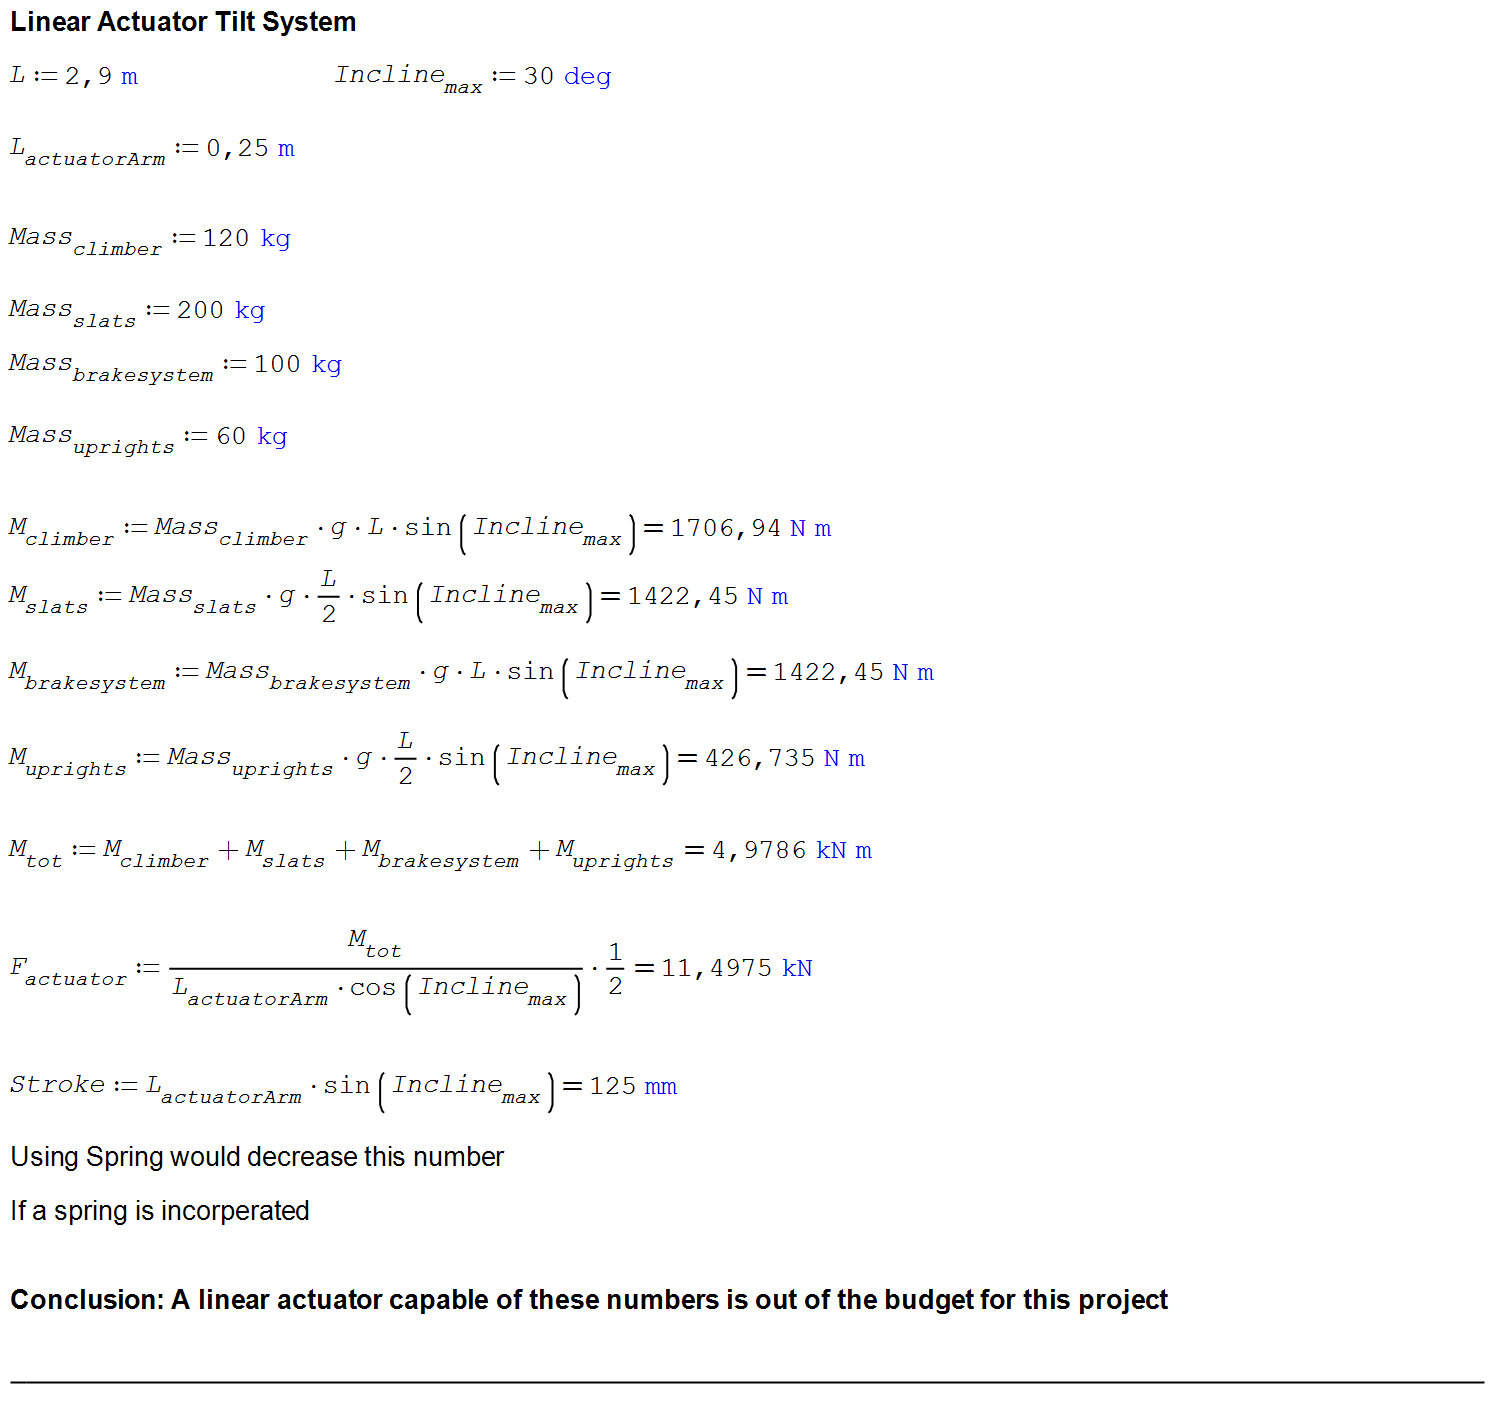
\includegraphics[width=1\linewidth]{chaps-append/calcs/linear_actuator_calcs.png}
\end{figure}

\section{Double Gear Down System Calculations}
\label{calcs:incline-system}

\begin{figure}[H]
    \centering
    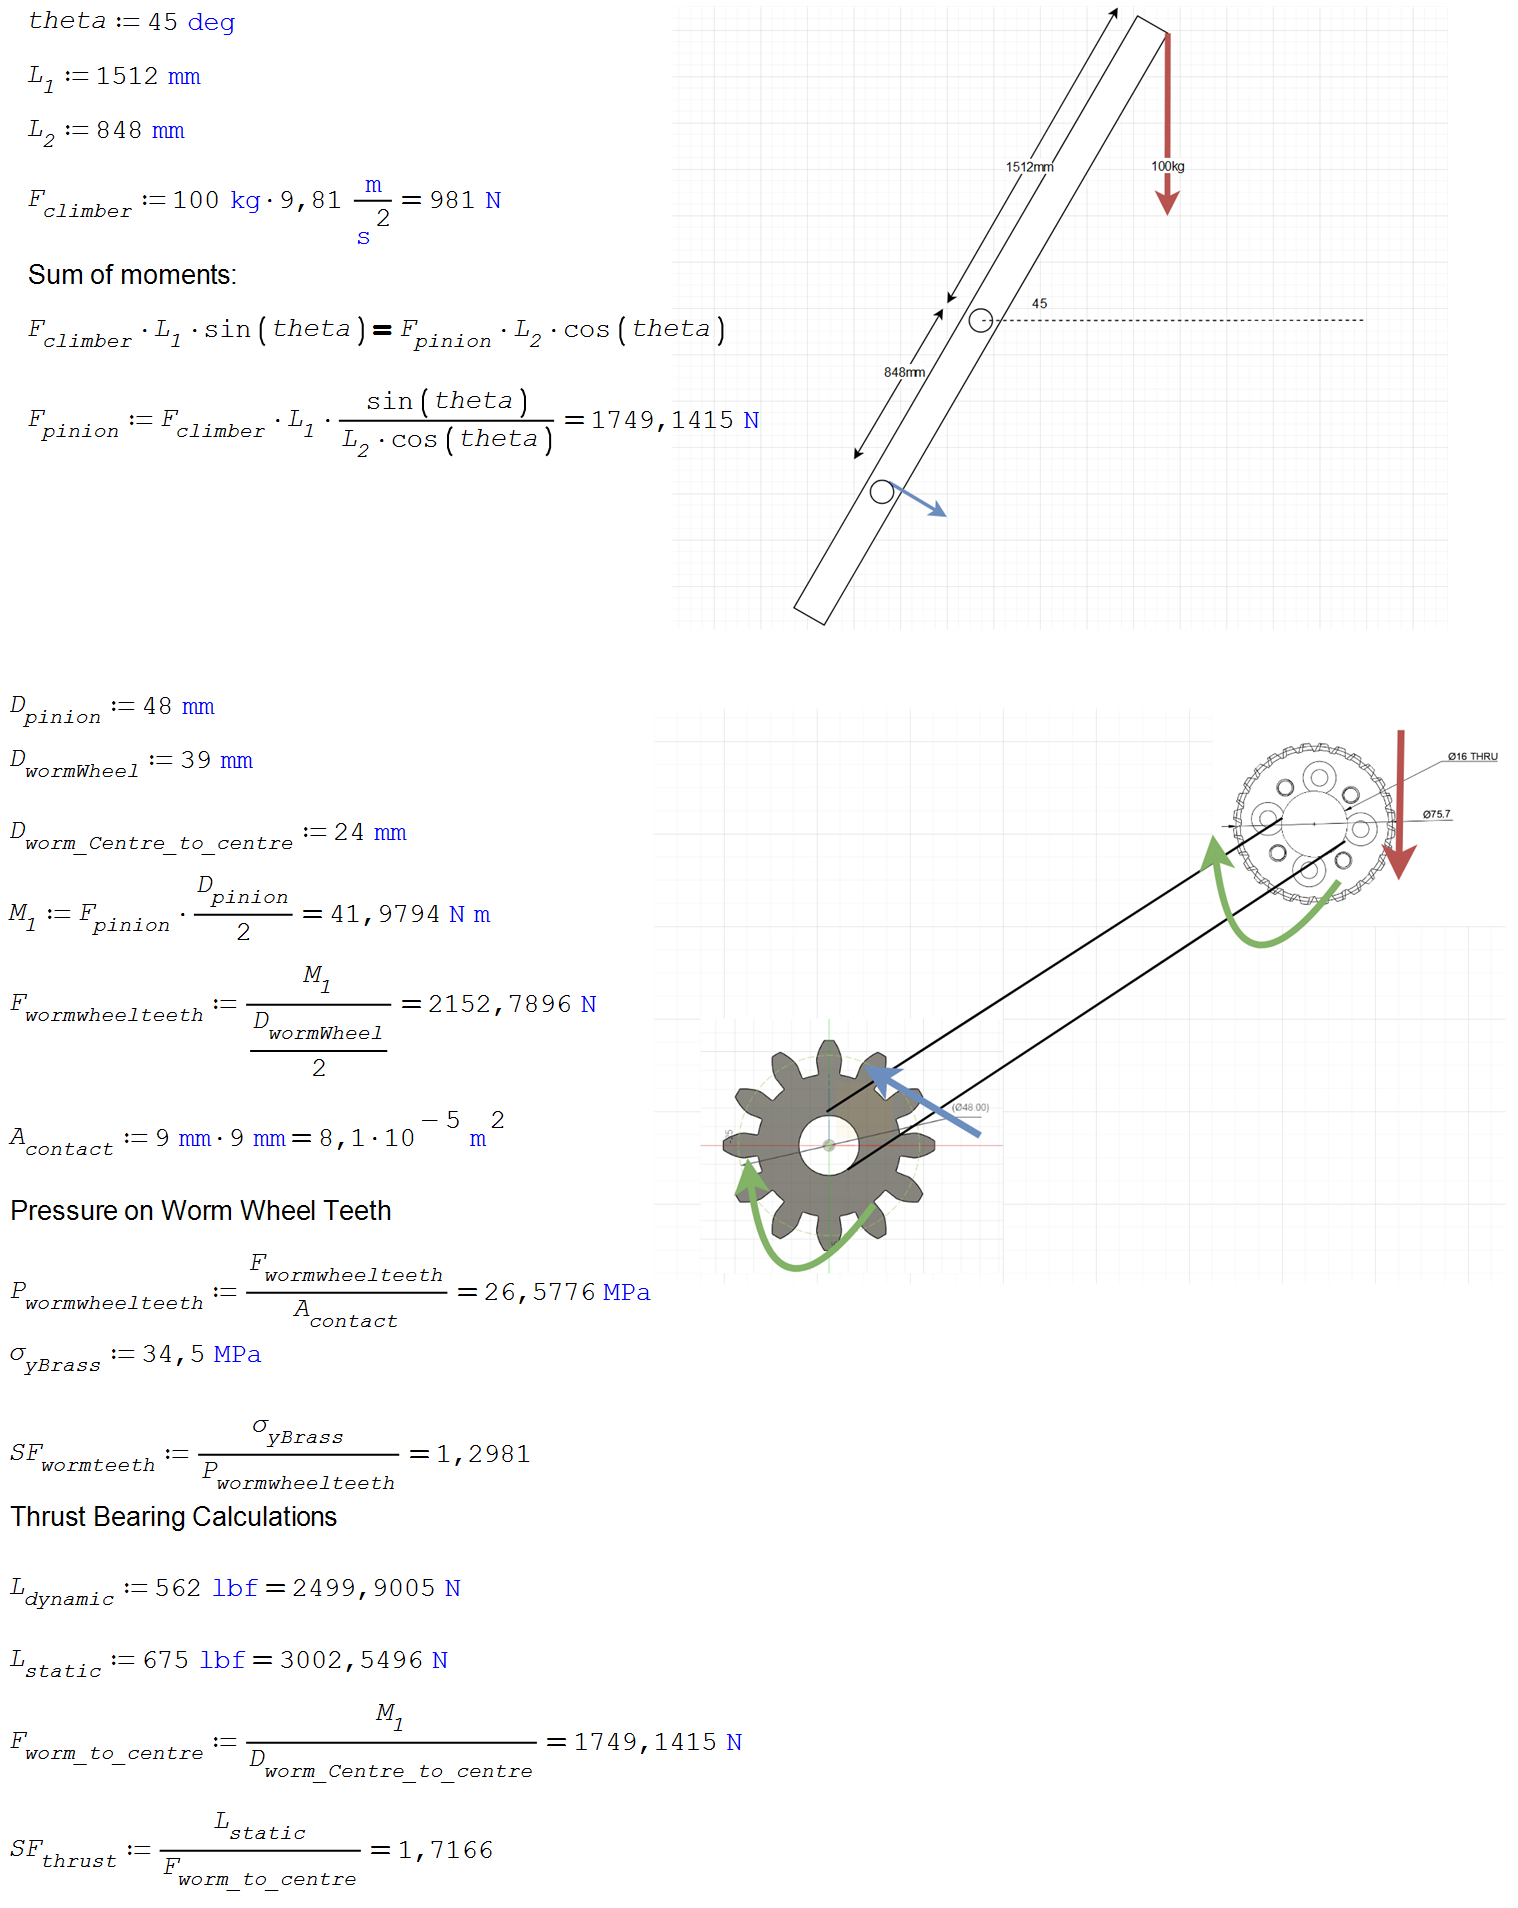
\includegraphics[width=1\linewidth]{chaps-append/calcs/tilting_max_torque_calcs.png}
\end{figure}
\begin{figure}[H]
    \centering
    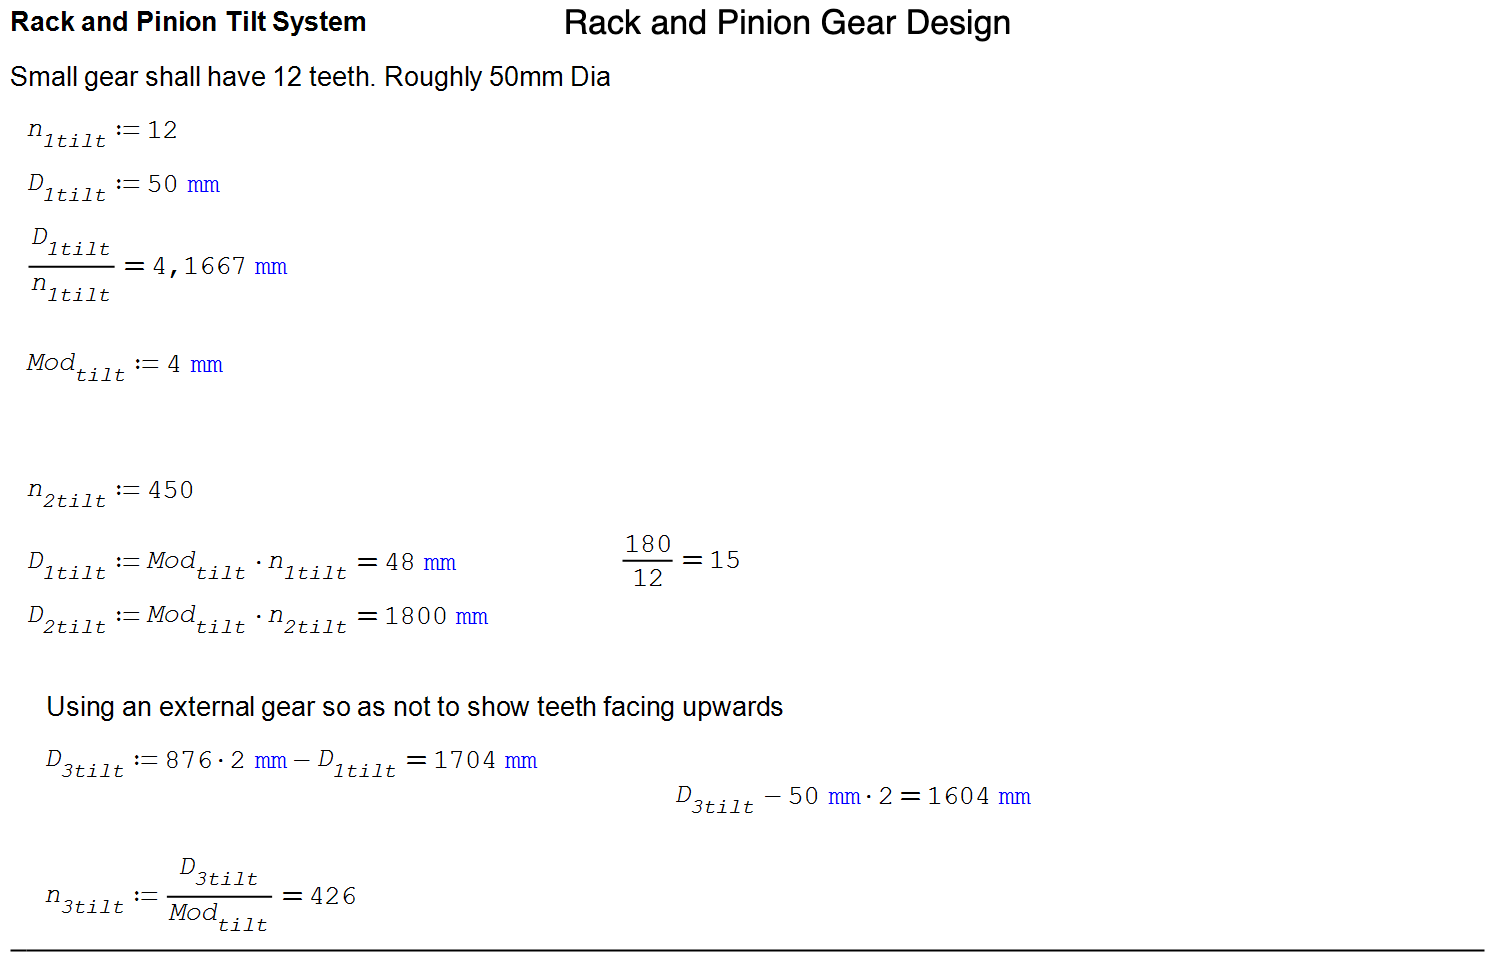
\includegraphics[width=1\linewidth]{chaps-append/calcs/rack_pinion_calcs.png}
\end{figure}

\subsection*{Safety Factor Calculation for Pinion Teeth}
\label{calcs:pinion-SF}
\small % Reduce font size for compactness

Given the following parameters:
\begin{itemize}
    \item Applied load: \( F = 1.75 \, \text{kN} = 1750 \, \text{N} \)
    \item Pitch radius: \( r_{\text{pinion}} = 24 \, \text{mm} \)
    \item Face width: \( b = 6 \, \text{mm} \)
    \item Module: \( m = 4 \, \text{mm} \)
    \item Material: Mild steel (\( \sigma_{\text{yield}} = 250 \, \text{MPa} \))
    \item Lewis form factor: \( Y \approx 0.3 \)
\end{itemize}

The bending stress is calculated using the Lewis equation:
\[
\sigma_{\text{bending}} = \frac{F \cdot r_{\text{pinion}}}{b \cdot m \cdot Y}
\]
Substituting the values:
\[
\sigma_{\text{bending}} = \frac{1750 \cdot 24}{6 \cdot 4 \cdot 0.3} = \frac{42000}{7.2} = 5833.33 \, \text{kPa} = 5.83 \, \text{MPa}
\]

Now, the safety factor is:
\[
\text{SF} = \frac{\sigma_{\text{yield}}}{\sigma_{\text{bending}}} = \frac{250 \, \text{MPa}}{5.83 \, \text{MPa}} \approx 42.88
\]

Thus, the safety factor for the pinion teeth is approximately \( \text{SF} \approx 42.88 \), indicating a very high safety margin under the given load.

\normalsize % Return to normal font size

\section{Stepper Motor Calculations}
\label{calcs:stepper-motor}

\small % Reduce font size for compactness

\subsection*{Torque Required for Tilting}


\[
T_{\text{shaft}} = 42 \, \text{Nm}, \quad \text{Worm Gear Ratio:} \, 28:1
\]

\subsection*{Gear Ratio Calculations}

\[
T_{\text{motor}} = \frac{T_{\text{shaft}}}{\text{Gear Ratio}} = \frac{42}{28} = 1.5 \, \text{Nm}
\]
\[
N_{\text{motor}} = 80 \, \text{rpm} = 8.377 \, \text{rad/s}
\]
\[
u_{\text{tot}} = u_{\text{tilt1}} \cdot u_{\text{tilt2}} = 16.67 \cdot 28 = 466.76
\]
\[
T_{\text{stepper}} = \frac{M_{\text{tilt}}}{u_{\text{tot}}} = \frac{874.03}{466.76} = 1.87 \, \text{Nm}
\]

\subsection*{Travel Time to Max Incline}

\[
\text{Travel angle} = 45^\circ + 15^\circ = 60^\circ
\]
\[
N_{\text{tilt}} = \frac{N_{\text{motor}}}{u_{\text{tilt1}} \cdot u_{\text{tilt2}}} = \frac{80}{466.76} = 0.171 \, \text{rpm}
\]
\[
t_{\text{tilt}} = \frac{\text{Travel angle}}{360^\circ} \cdot \frac{60}{N_{\text{tilt}}} = \frac{60^\circ}{360^\circ} \cdot \frac{60}{0.171} \approx 29.24 \, \text{seconds}
\]

Speed and torque well within range of Nema 23 stepper motor which has a max holding torque of 2Nm and speed of 1000 rpm.

\normalsize % Return to normal font size

\section{Worm Gear Bracket FEM Analysis}
\label{calcs:worm-bracket-fem}
Finite Element Method (FEM) analysis was conducted on the worm gear bracket system using the maximum calculated force from Section~\ref{calcs:incline-system}. The simulation was run with the force applied both upwards and downwards. As shown in Figure~\ref{fig:FEM-incline-brackets}, the maximum stress observed in the system is 209\,MPa. Given the yield strength of mild steel is approximately 250\,MPa, the safety factor for the bracket system is calculated as:

\[
\text{Safety Factor} = \frac{\sigma_{\text{yield}}}{\sigma_{\text{max}}} = \frac{250 \, \text{MPa}}{209 \, \text{MPa}} \approx 1.2
\]

This indicates that the worm gear bracket system operates with a safety factor of approximately 1.2, which is adequate for the specified load conditions.



\section{Incline Shaft FEM Analysis}
\label{calcs:incline-shaft}
The torque values calculated above were used in a Fusion 360 static FEM analysis with the following results:
\begin{figure}[H]
    \centering
    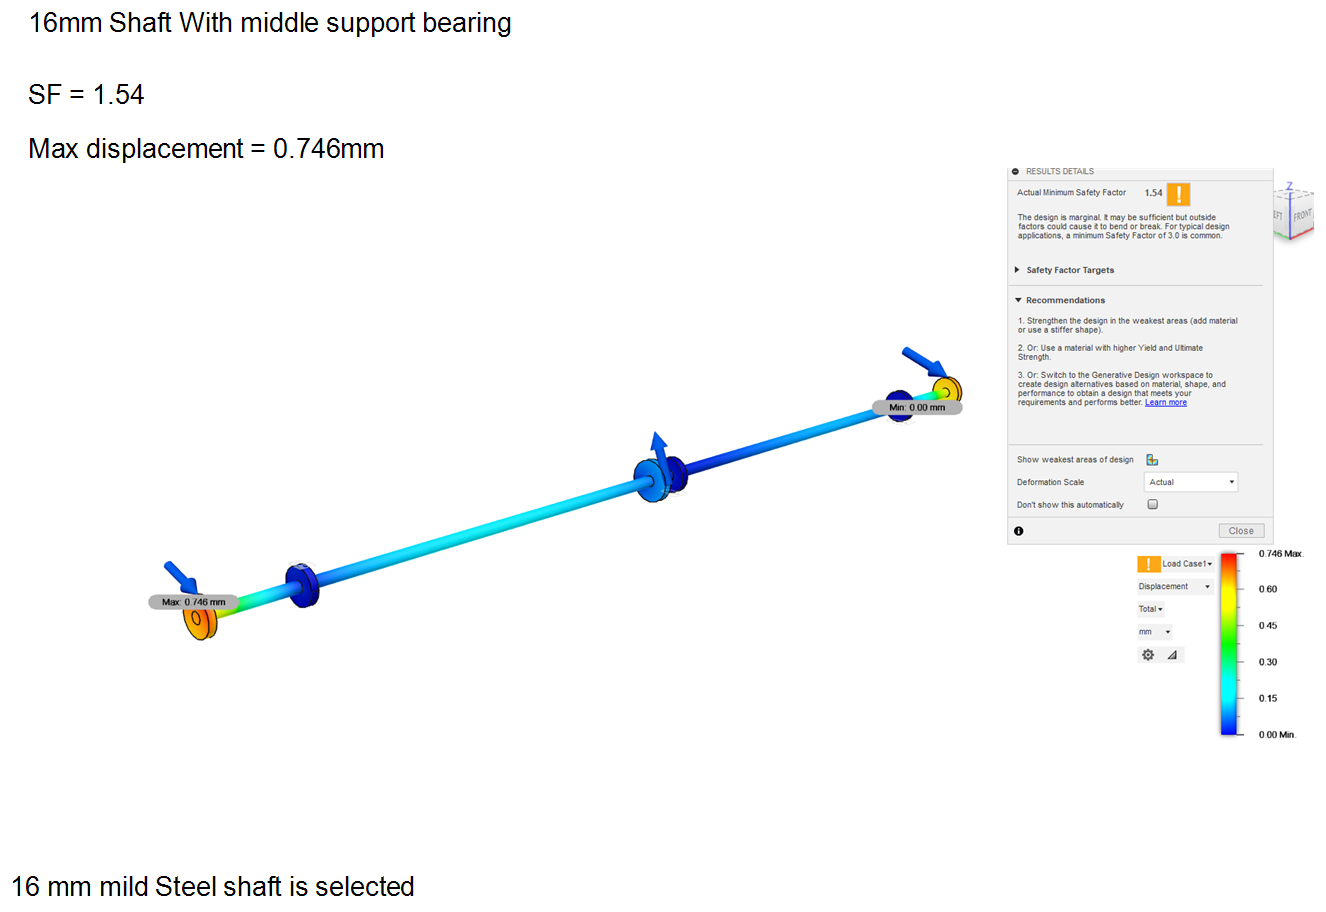
\includegraphics[width=1\linewidth]{chaps-append/calcs/tilt_shaft_FEM.png}
\end{figure}




\chapter{Braking System Calculations}
\label{appx:braking-calcs}

\section{Brake Disk Heating Analysis with Natural Convection}
\label{calcs:brake-disk-heat}
This section analyzes the brake disk's temperature rise due to frictional heating using a lumped mass model and a detailed simulation from Fusion 360, both assuming natural convection as the primary cooling mechanism.

\subsection*{Lumped Mass Model}
A lumped mass approach was used to estimate the temperature rise of the brake disk. 
This analysis was based on the lumped mass method, as described in \cite{cengel2015heat}.
The parameters for the analysis are:
\begin{itemize}
    \item Mass: \( m = 0.054 \, \text{kg} \)
    \item Specific heat: \( c_p = 897 \, \frac{\text{J}}{\text{kg°C}} \)
    \item Surface area: \( A = 0.02997 \, \text{m}^2 \)
    \item Heat input: \( Q_{\text{in}} = 1200 \, \text{W} \)
    \item Natural convection coefficient: \( h_{\text{natural}} = 25 \, \frac{\text{W}}{\text{m}^2 \cdot \text{K}} \)
\end{itemize}

The lumped mass heat balance equation is:
\[
Q_{\text{in}} - Q_{\text{out}} = m c_p \frac{dT}{dt}, \quad Q_{\text{out}} = h_{\text{natural}} A (T - T_{\text{ambient}})
\]

The following Python script was used to calculate the temperature rise over a period of 300 seconds:

\subsection*{Python Script}

\small % Smaller font size for the Python script
\begin{verbatim}
import numpy as np
import matplotlib.pyplot as plt

# Constants
m_brake = 0.054  # kg
c_brake = 897  # J/kg°C
h_natural = 25  # W/m²·K
A_brake = 0.02997  # m²
Q_in = 1200  # W
T_ambient = 300  # K

# Time parameters
time = np.linspace(0, 300, 1000)  # 300 seconds
dt = time[1] - time[0]
T = np.zeros_like(time)
T[0] = T_ambient

# Calculate temperature rise over time
for i in range(1, len(time)):
    Q_out = h_natural * A_brake * (T[i-1] - T_ambient)
    dTdt = (Q_in - Q_out) / (m_brake * c_brake)
    T[i] = T[i-1] + dTdt * dt

# Plot the temperature rise over time
plt.plot(time, T - 273.15, label="Natural Convection")
plt.axhline(y=650, color='blue', linestyle='--', label="Max Allowable Temp (650°C)")
plt.xlabel('Time (s)')
plt.ylabel('Temperature (°C)')
plt.title('Brake Disk Temperature Rise Over Time')
plt.legend()
plt.grid(True)
plt.show()
\end{verbatim}
\normalsize % Return to normal font size

\begin{figure}[H]
    \centering
    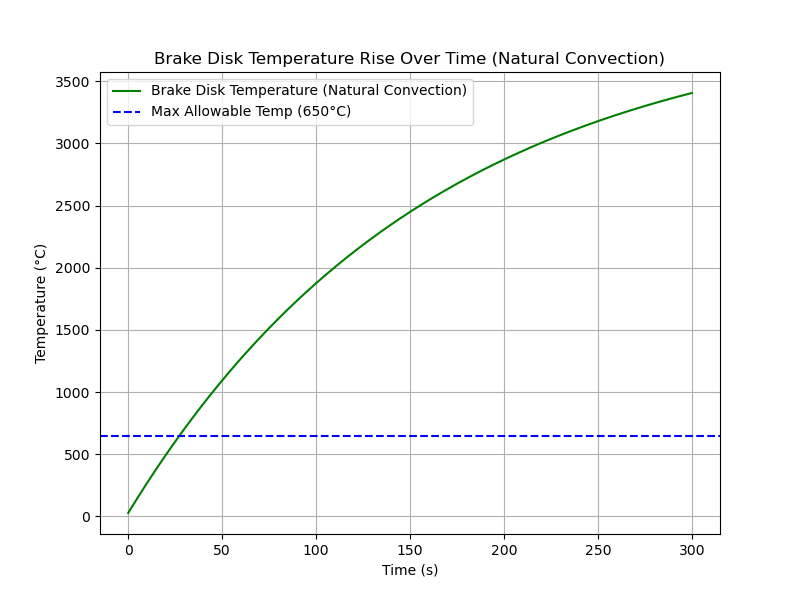
\includegraphics[width=0.8\linewidth]{chaps-append/calcs/disk_brake_heat_python.png}
\end{figure}


\begin{figure}[H]
    \centering
    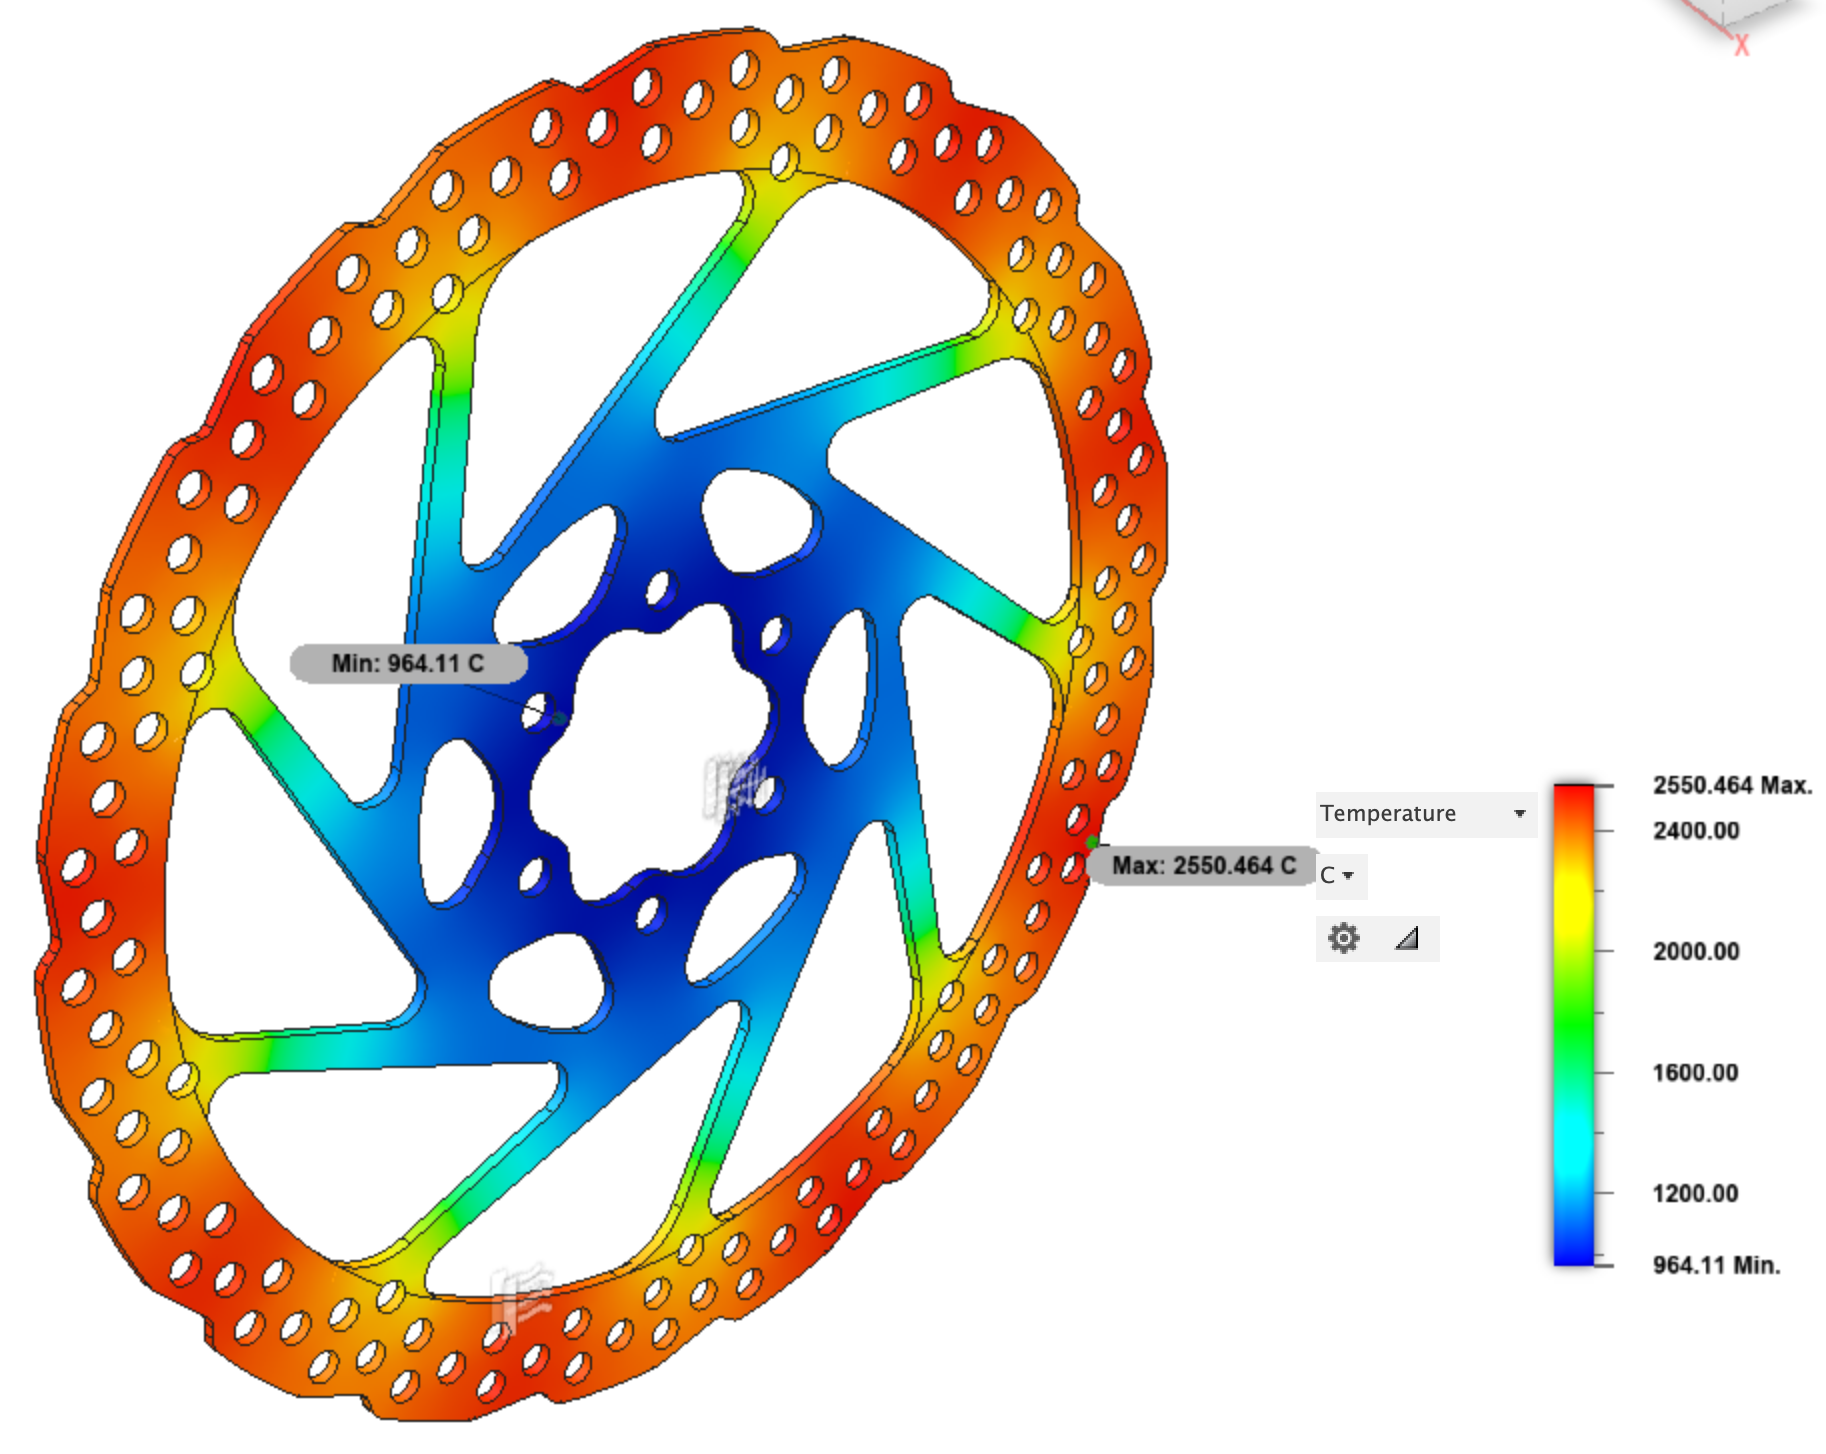
\includegraphics[width=0.8\linewidth]{chaps-append/calcs/disk_brake_heat_simulation.png}
    \caption{Fusion 360 Simulation: Brake Disk Temperature with Natural Convection}
    \label{fig:brake-fusion-simulation}
\end{figure}


\section{Main Shaft Calculations}
\label{calcs:main_braking_shaft}

\begin{figure}[H]
    \centering
    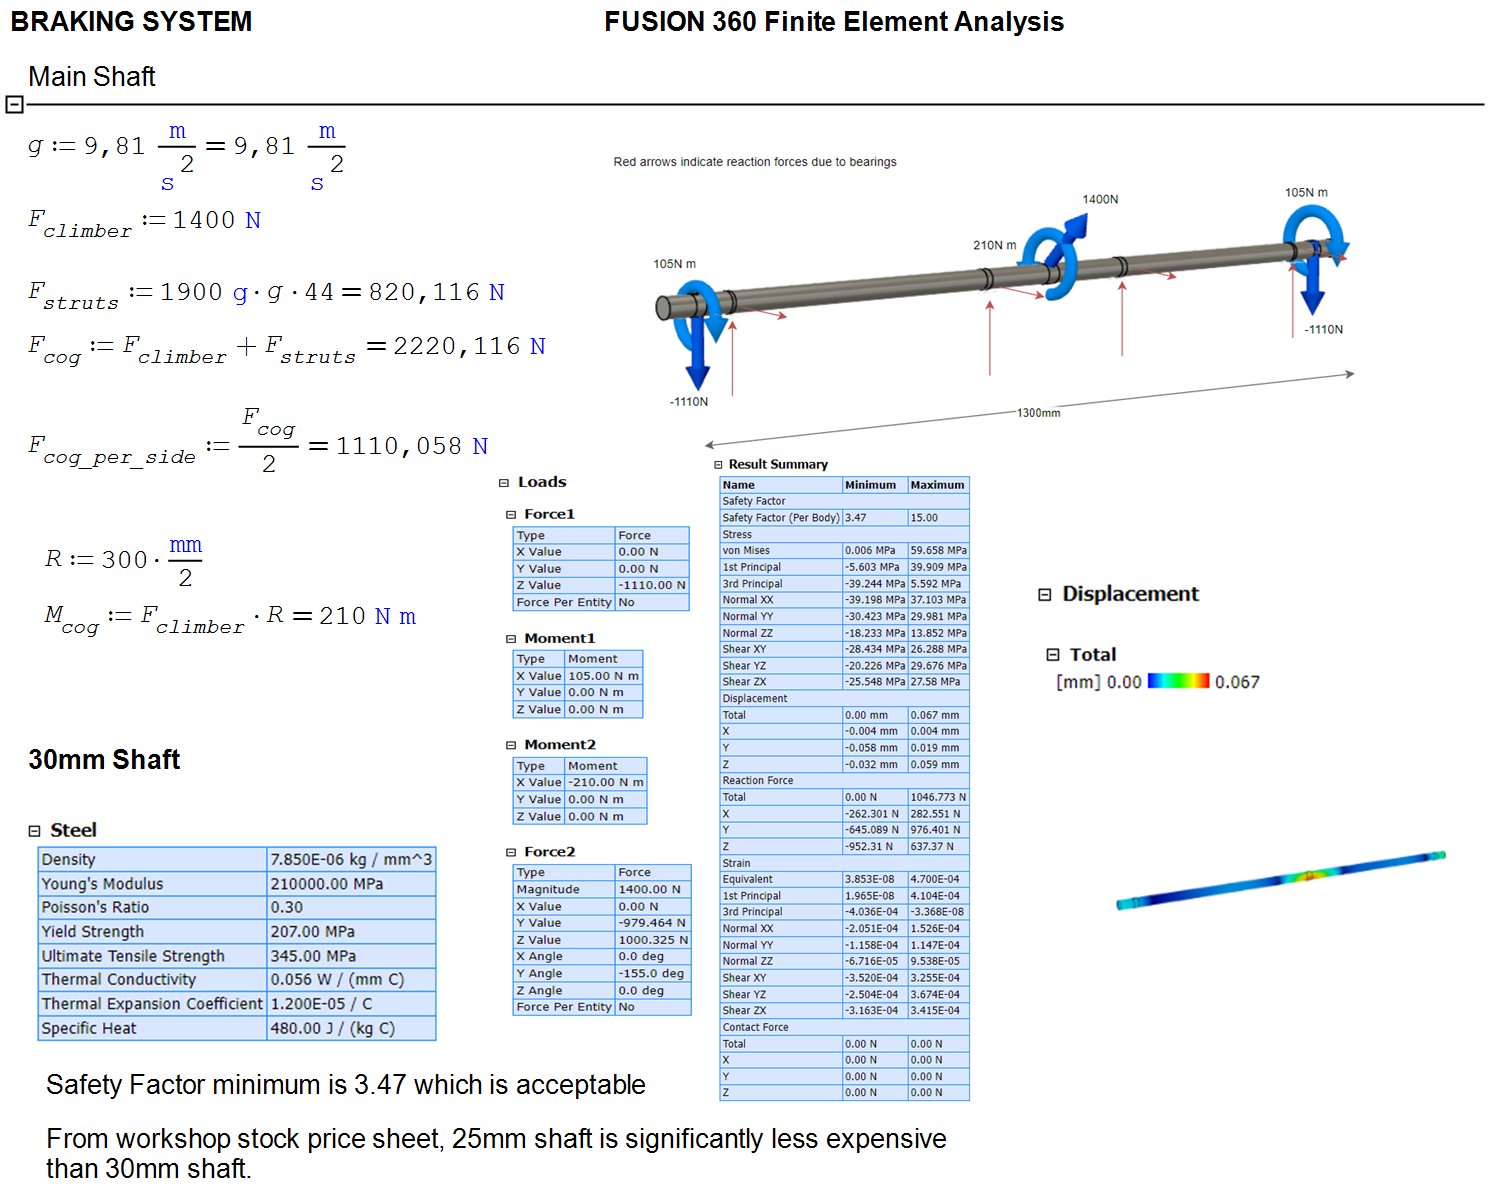
\includegraphics[width=0.9\linewidth]{chaps-append/calcs/main_shaft_calcs1.png}
\end{figure}

\begin{figure}[H]
    \centering
    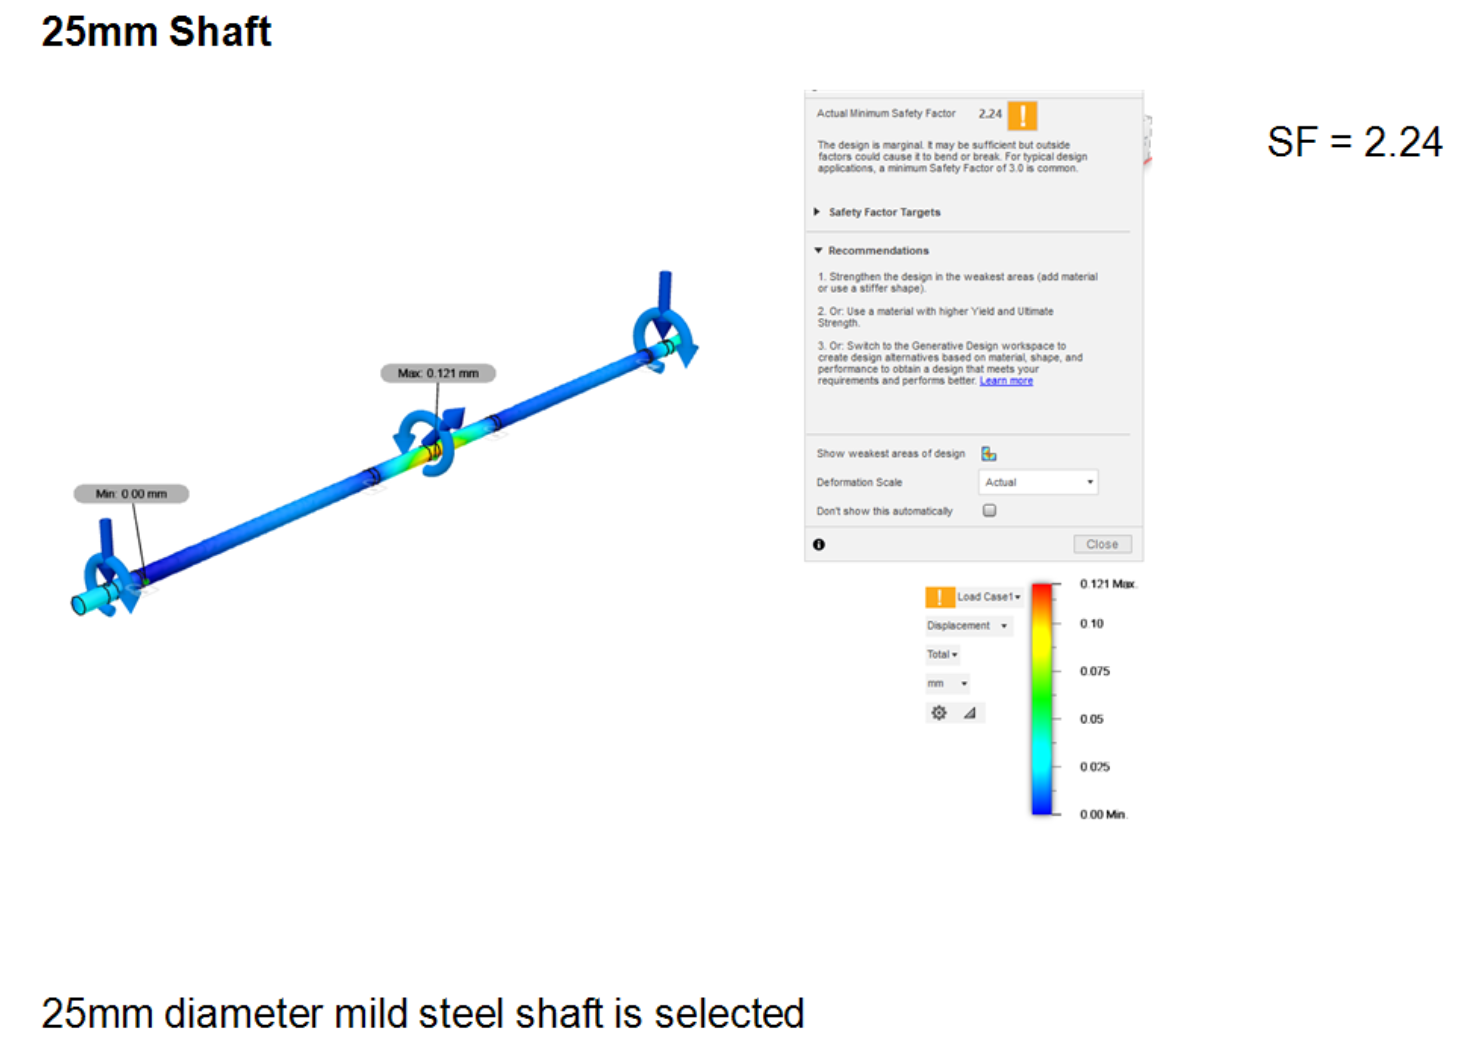
\includegraphics[width=0.7\linewidth]{chaps-append/calcs/main_shaft_calcs_2.png}
\end{figure}

\section{Brackets and Bearings Calculations}
\label{calcs:brackets_bearings}

\subsection*{Laser Cut Brackets}

\begin{figure}[H]
    \centering
    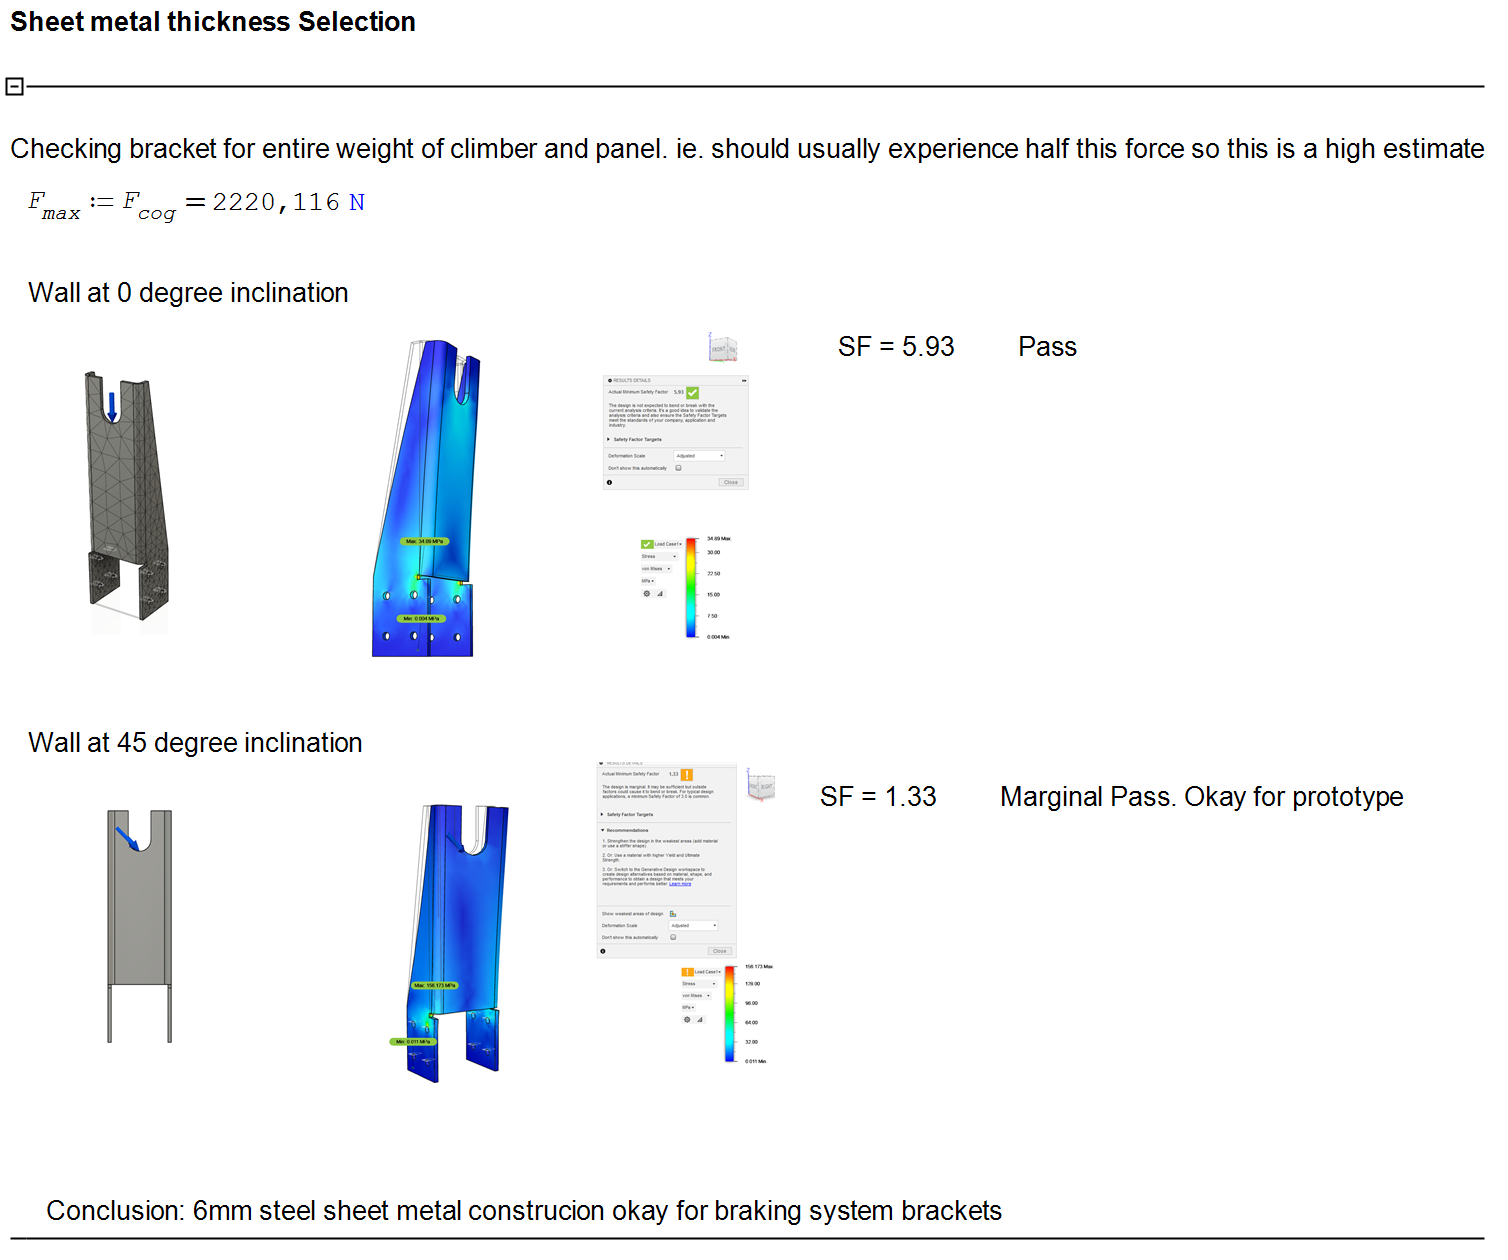
\includegraphics[width=1\linewidth]{chaps-append/calcs/FEM_brackets.png}
\end{figure}

\subsection*{Main Shaft Bearing Verification}

Assuming the bearings transfer all the force from the shaft to the brackets, the maximum force is calculated as:

\[
F_{\text{max}} = 2220\ \text{N}
\]

Using a \textbf{Koyo UCF205 Flange unit bearing} with a basic load rating of \( C_{0r} = 7.85\ \text{kN} \), the bearing can safely handle the applied load.

\section{Motor and Belt Drive System Calculations}
\label{calcs:motor_belt}

\subsection*{Mechanical Losses in Rotating System}

There is a significant amount of torque lost due to friction in the bearings and panels sliding through aluminum channels. Accounting for these frictional losses reduces the torque needed to brake the system and allows for a simpler motor and pulley system.

First, calculate the gravitational force due to the wood panels:

\[
F_{\text{woodPanels}} = N_{\text{panels}} \times m_{\text{panel}} \times g = 41 \times 2\ \text{kg} \times 9.81\ \text{m/s}^2 = 803.22\ \text{N}
\]

Where:
\begin{itemize}
    \item \( N_{\text{panels}} = 41 \) is the number of panels.
    \item \( m_{\text{panel}} = 2\ \text{kg} \) is the mass of each panel.
    \item \( g = 9.81\ \text{m/s}^2 \) is the acceleration due to gravity.
\end{itemize}

Next, consider the weight of the climber (assuming a maximum climber mass of 90\,kg):

\[
F_{\text{climber\_low}} = m_{\text{climber\_low}} \times g = 90\ \text{kg} \times 9.81\ \text{m/s}^2 = 882.9\ \text{N}
\]

The torque due to the climber's weight is:

\[
M_{\text{climber\_low}} = F_{\text{climber\_low}} \times r = 882.9\ \text{N} \times 1\ \text{m} = 882.9\ \text{Nm}
\]

Assuming rotational equilibrium, the normal force on each wall due to the climber is:

\[
F_{\text{N\_W}} = \frac{M_{\text{climber\_low}}}{2 \times L} = \frac{882.9\ \text{Nm}}{2 \times 0.85\ \text{m}} = 519.35\ \text{N}
\]

Where \( L = 0.85\ \text{m} \) is the horizontal distance from the pivot to the point of contact.

The coefficient of dynamic friction between aluminum and nylon is:

\[
\mu_{\text{alu\_nylon}} = 0.25
\]

The frictional force at one contact point is:

\[
F_{\text{f,single}} = F_{\text{N\_W}} \times \mu_{\text{alu\_nylon}} = 519.35\ \text{N} \times 0.25 = 129.84\ \text{N}
\]

The total frictional force due to all four contact points is:

\[
F_{\text{f}} = 4 \times F_{\text{f,single}} = 4 \times 129.84\ \text{N} = 519.35\ \text{N}
\]

The braking torque produced by this friction is:

\[
T_{\text{friction}} = F_{\text{f}} \times \frac{D}{2}
\]

Assuming the diameter \( D \) is such that \( T_{\text{friction}} = 64.92\ \text{Nm} \), we proceed with this value.

The torque required on the shaft to overcome the climber's weight, accounting for friction, is:

\[
T_{\text{shaft}} = F_{\text{climber\_low}} \times \frac{D}{2} - T_{\text{friction}} = 45.44\ \text{Nm}
\]

This reduced torque requirement allows for the selection of a less powerful motor, optimizing cost and efficiency.

\subsection*{Torque Reduction Ratio Calculation}

The required torque at the shaft is:

\[
T_{\text{shaft}} = 45.44\ \text{Nm}
\]

The motor's continuous torque is:

\[
T_{\text{motor}} = 10\ \text{Nm}
\]

Therefore, the necessary gear reduction ratio is:

\[
R = \frac{T_{\text{shaft}}}{T_{\text{motor}}} = \frac{45.44\ \text{Nm}}{10\ \text{Nm}} = 4.544
\]

A gear reduction ratio of approximately 5:1 is required. This justifies the selection of the 90-tooth to 18-tooth pulley system, providing the needed gear ratio.

\subsection*{Motor Selection}

Based on the torque and speed requirements calculated, the motor must provide a continuous torque of at least 10\,Nm and operate at speeds up to 1000\,rpm. The \textbf{MiGE 130ST-M10010} motor was selected due to its specifications matching these requirements.

\paragraph{Motor Requirements}

- \textbf{Continuous torque required after gear reduction}:

\[
T_{\text{motor}} = \frac{T_{\text{shaft}}}{R} = \frac{45.44\ \text{Nm}}{5} = 9.09\ \text{Nm}
\]

- \textbf{Speed required at motor shaft}:

\[
n_{\text{motor}} = n_{\text{shaft}} \times R = 159\ \text{rpm} \times 5 = 795\ \text{rpm}
\]

\paragraph{Motor Specifications}

- \textbf{Continuous torque}: 10\,Nm
- \textbf{Rated speed}: 1000\,rpm

These specifications meet or exceed the calculated requirements, confirming the suitability of the MiGE 130ST-M10010 motor for this application.

\begin{figure}[H]
    \centering
    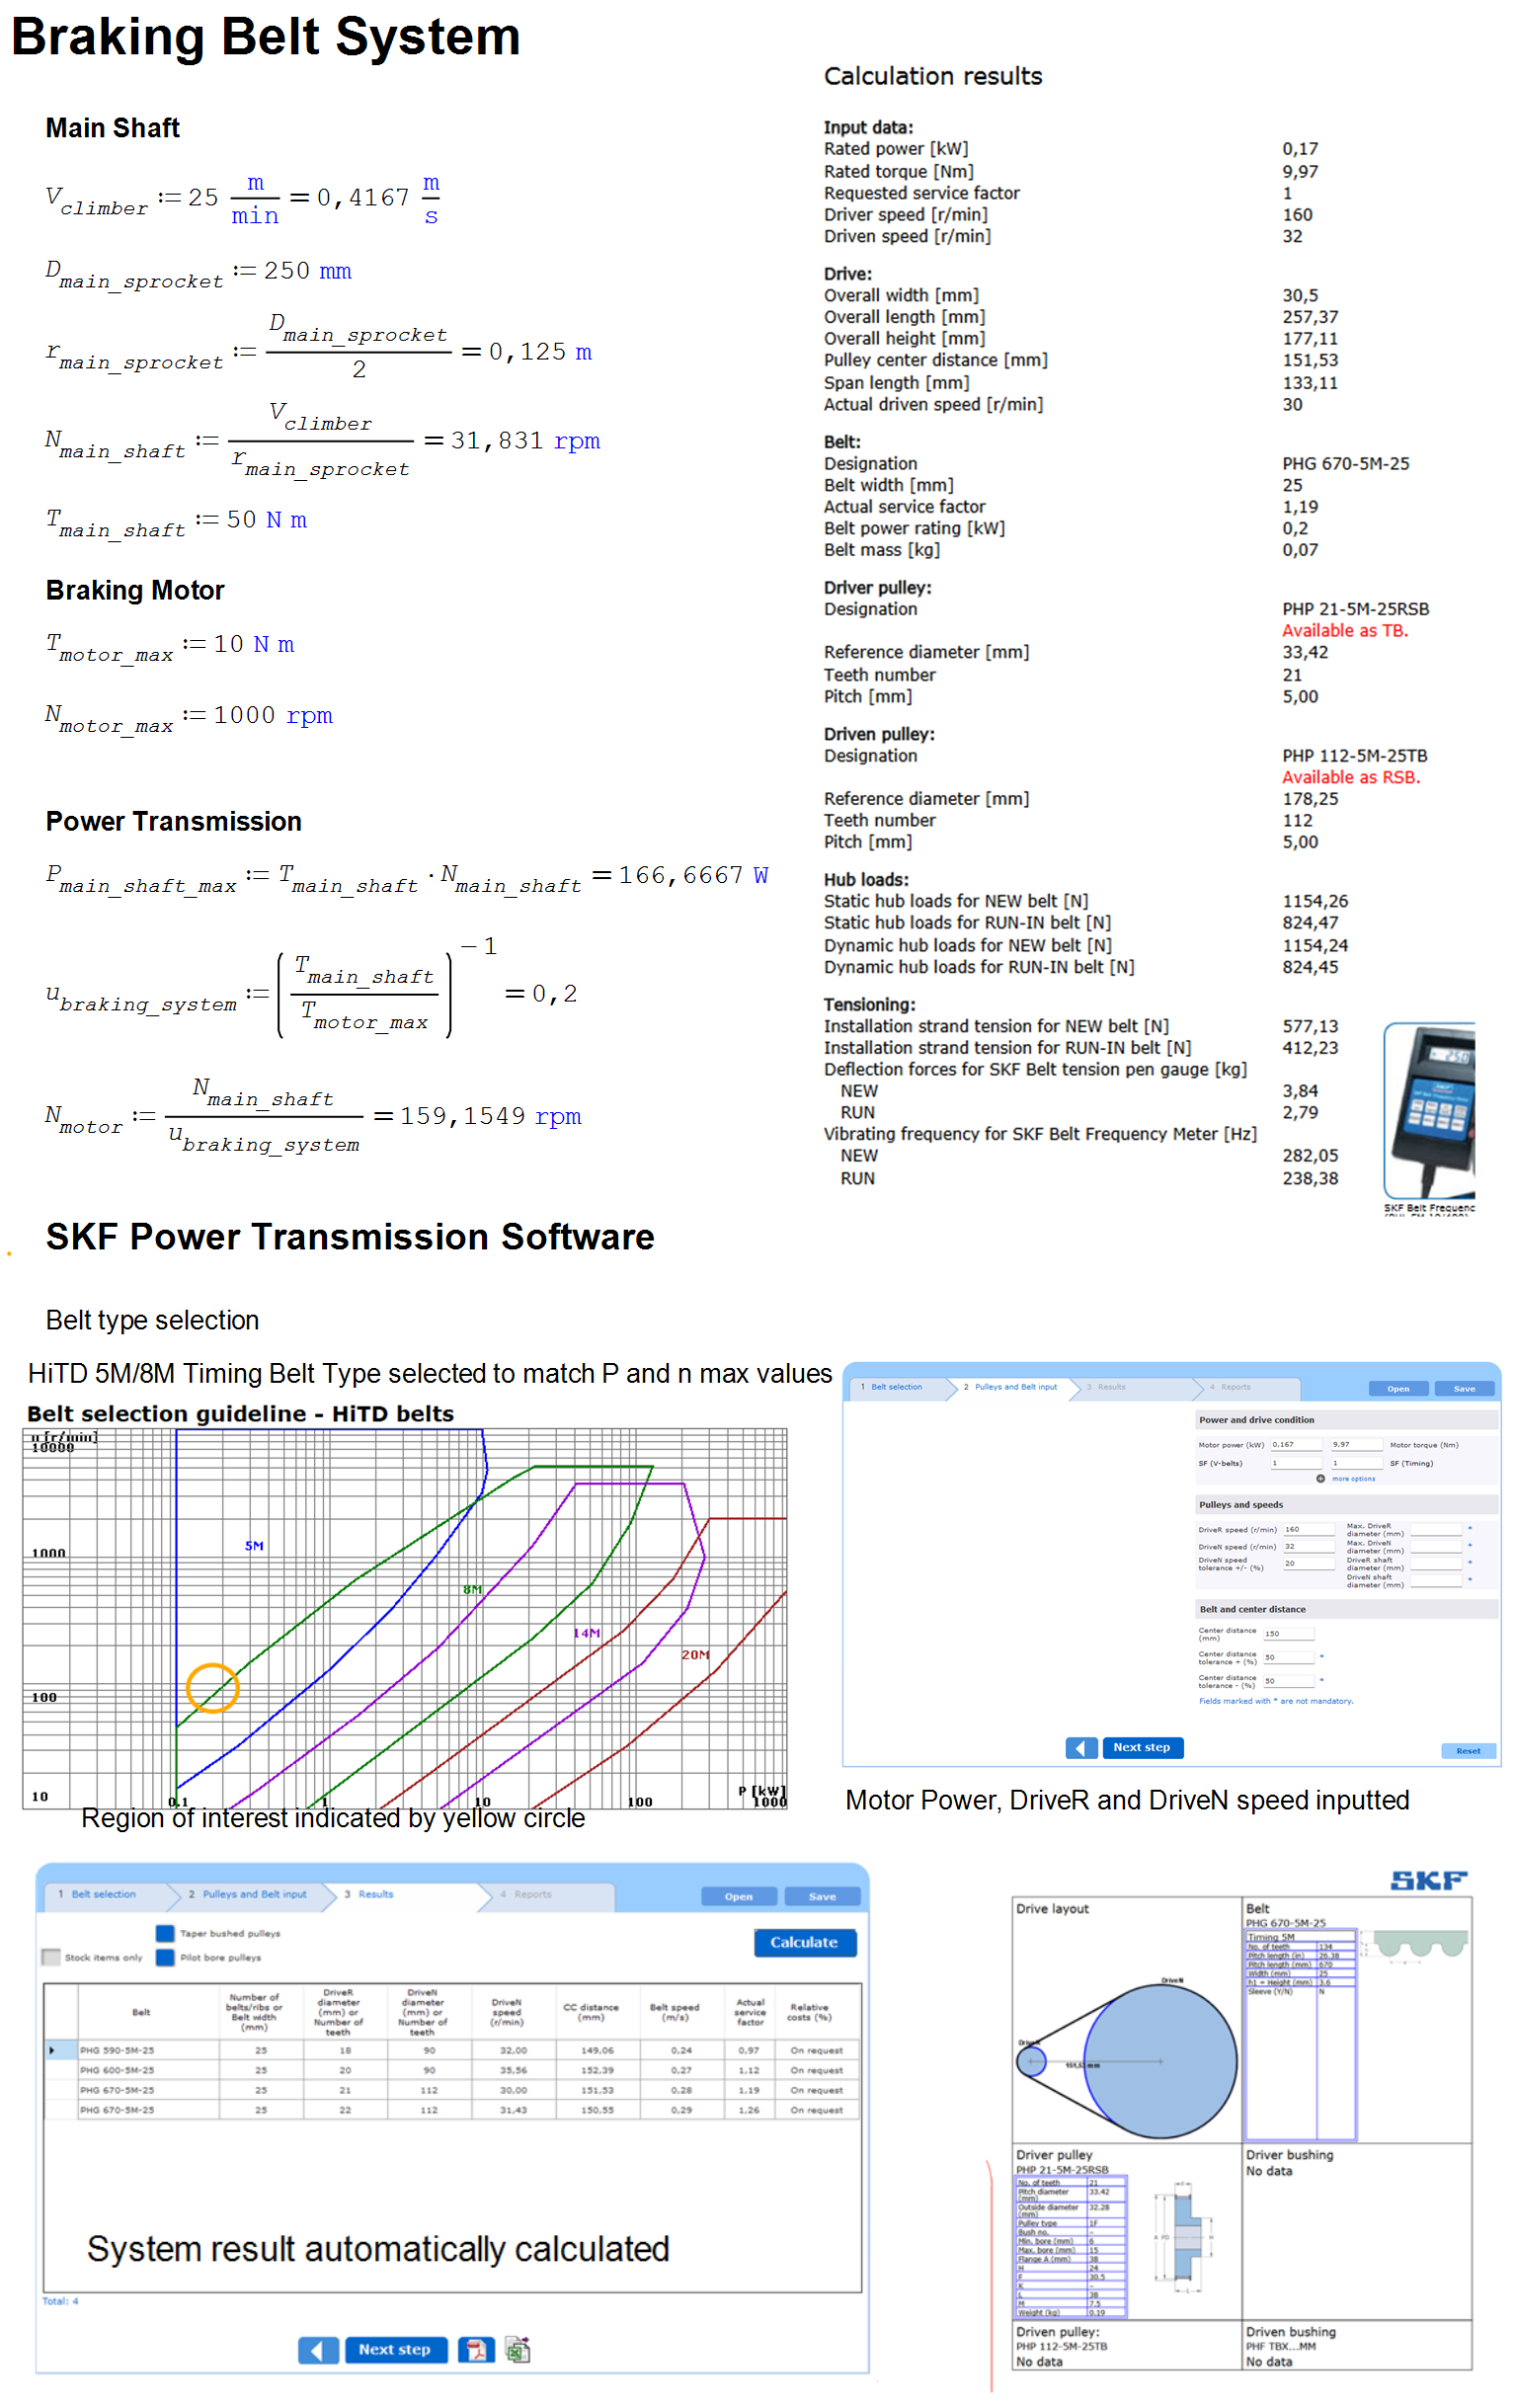
\includegraphics[width=1\linewidth]{chaps-append/calcs/belt_selection.png}
\end{figure}

\section{Braking Resistor Design}
\label{calcs:braking_resistor}

To determine the appropriate braking resistor, we calculate the voltage at the maximum motor speed using the voltage constant of the motor.

The voltage constant of the MiGE 130ST-M10010 motor is:

\[
K_v = 140\ \text{V/krpm}
\]

Assuming the maximum motor speed in this application is:

\[
n_{\text{max}} = 159\ \text{rpm}
\]

Converting rpm to krpm:

\[
n_{\text{max, krpm}} = \frac{159\ \text{rpm}}{1000} = 0.159\ \text{krpm}
\]

Calculating the maximum generated voltage:

\[
V_{\text{max\_speed}} = K_v \times n_{\text{max, krpm}} = 140\ \text{V/krpm} \times 0.159\ \text{krpm} = 22.26\ \text{V}
\]

The braking power remains:

\[
P_{\text{brake}} = P_{\text{gen}} \times 1.5 = 227.22\ \text{W}
\]

The current through the braking resistor is:

\[
I_{\text{brake}} = \frac{P_{\text{brake}}}{V_{\text{max\_speed}}} = \frac{227.22\ \text{W}}{22.26\ \text{V}} = 10.21\ \text{A}
\]

Finally, the braking resistor value is calculated as:

\[
R_{\text{brake}} = \frac{V_{\text{max\_speed}}}{I_{\text{brake}}} = \frac{22.26\ \text{V}}{10.21\ \text{A}} = 2.18\ \Omega
\]



\chapter{Rotating Surface Calculations}

\section{Chain Calculations}
\label{calcs:chain}
\begin{figure}[H]
    \centering
    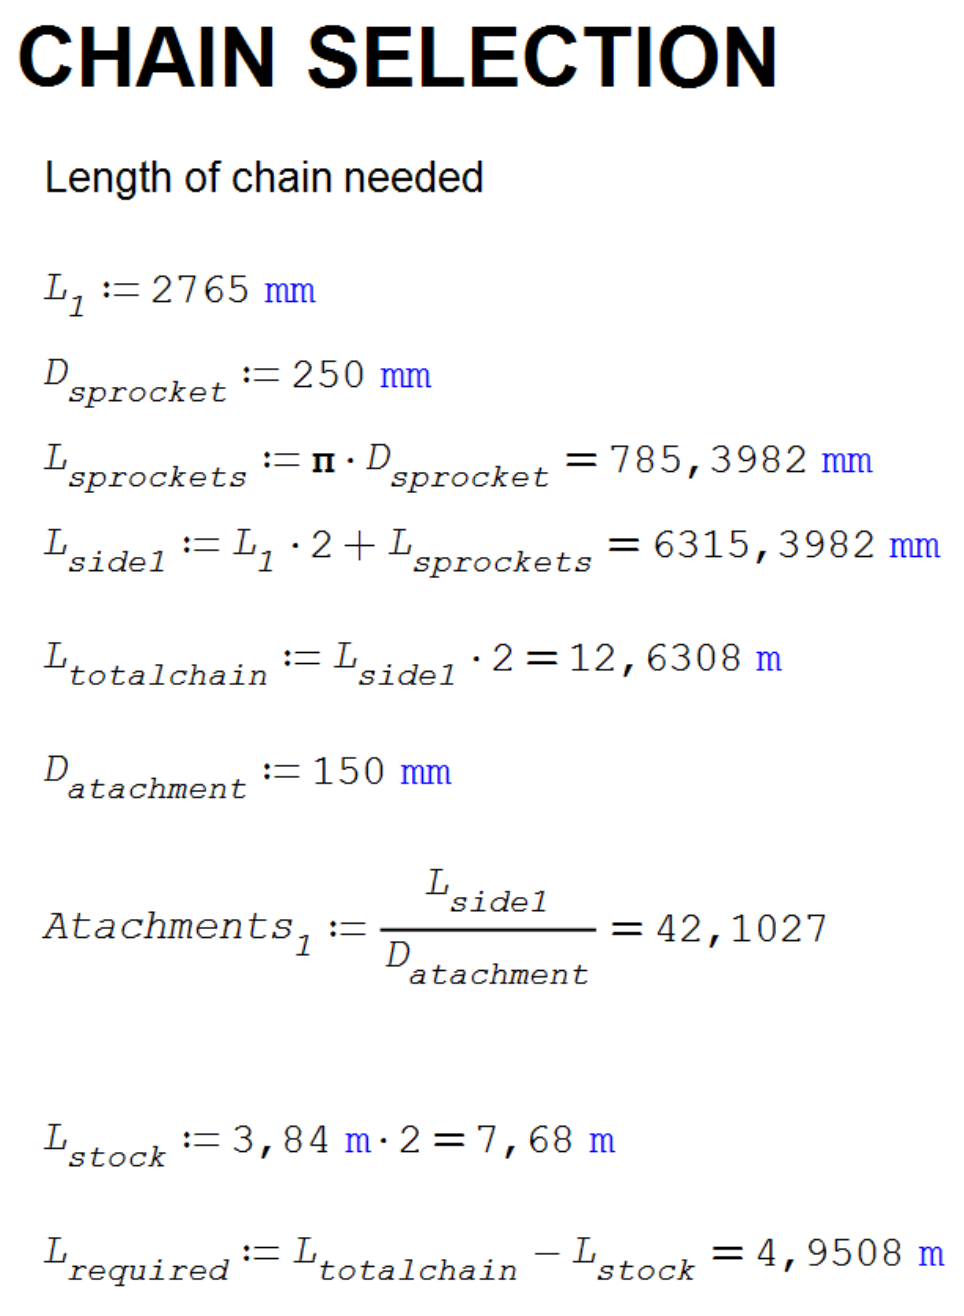
\includegraphics[width=0.8\linewidth]{chaps-append/calcs/chain-length-calcs.png}
\end{figure}



